\chapter{Communication Protocol} \label{sec:tinyframe}

GEX can be controlled through a hardware \gls{UART}, the \gls{USB} or over a wireless link. To minimize the firmware complexity, all the three connection methods are handled by the same protocol stack and are functionally interchangeable.

The communication is organized in transactions. A transaction consists of one or more messages going in either direction. Messages can be stand-alone, or chained with a response or a follow-up message using the transaction ID. Both peers, GEX and the client application running on the host PC, are equal in the communication: either side can independently initiate a transaction at any time.

GEX uses a framing library \textit{TinyFrame}, developed likewise by the author but kept as a separate project for easier re-use in different applications. The library implements frame building and parsing, checksum calculation and a system of message listeners.

\section{Frame Structure}

Message frames have the following structure (all little-endian):

\begin{boxedpayload}[``TinyFrame'' frame structure, as used in GEX]
	\cfield{u8} start-of-frame marker (0x01)
	\cfield{u16} frame ID
	\cfield{u16} payload length
	\cfield{u8} frame type
	\cfield{u8} header checksum	
	\cfield{u8[]} payload
	\cfield{u8} payload checksum (omitted for empty payloads)
\end{boxedpayload}

\iffalse
\begin{table}[h]
	\centering
	%\hspace{-1.5em}
	\begin{tabular}{rccccccc}
		\toprule
		\multicolumn{1}{c|}{} &
		\multicolumn{5}{c}{Header}&
		\multicolumn{2}{|c}{Body} \\
		\midrule
		%
		\textit{Field} &
			\textbf{SOF} &
			\textbf{Frame ID} &
			\makecell{ \Gape{\textbf{Payload}} \\ \Gape{\textbf{Length}} } &
			\makecell{ \textbf{Frame} \\ \textbf{type} } &
			\makecell{ \textbf{Header} \\ \textbf{checksum} } &
			\textbf{Payload} &
			\makecell{ \textbf{Payload} \\ \textbf{checksum} } \\
		%
		\midrule
		\textit{Bytes} &
			 1  &
			 2  &
			 2  &
			 1  &
			 1  &
			 ... &
			 1 \\
		%
		\bottomrule
	\end{tabular}
\end{table}
\fi

\textit{Frame ID}, which could be better described as \textit{Transaction ID}, uniquely identifies each transaction. The most significant bit is set to a different value in each peer to avoid ID conflicts, and the rest of the ID field is incremented with each initiated transaction.

\section{Message Listeners}

After sending a message that should receive a response, the peer registers an \textit{ID listener} with the ID of the sent message. A response reuses the original frame ID and when it is received, this listener is called to process it. ID listeners can also be used to receive multi-part messages re-using the original ID.

\textit{Frame type} describes the payload and does not have any prescribed format; the values are defined by application (here, GEX). A \textit{type listener} may be registered to handle all incoming messages with a given frame type. It works in a similar way to an ID listener and has a lower priority.

Each message can be handled by only one listener, unless it explicitly requests the message to be passed on to a lower priority one. Messages unhandled by any listener are given to a default listener, which can e.g. write an error to a debug log.

\section{Designated Frame Types}

The following table lists all frame types used by GEX. It is divided into four logical sections: General, Bulk Read/Write, Unit Access, and Settings.

\begin{table*}[h]
	\centering
	\begin{tabular}{clll}
		\toprule
		\textbf{Frame type} & \textbf{Function} & \textbf{Note} \\
		\midrule
		0x00 & Success & \textit{Payload depends on context} \\
		0x01 & Ping & \textit{GEX responds with Success and its version string} \\
		0x02 & Error & \textit{Payload contains the error message} \\
		\midrule
		0x03 & Bulk Read Offer & \textit{An offer of data to read using }0x04 \\
		0x04 & Bulk Read Poll & \textit{Requesting to read a block of data} \\
		0x05 & Bulk Write Offer & \textit{An offer to receive a bulk write transaction} \\
		0x06 & Bulk Data & \textit{Used for both reading and writing} \\
		0x07 & Bulk End & \textit{Marks the last ``Bulk Data'' frame} \\
		0x08 & Bulk Abort & \textit{} \\
		\midrule
		0x10 & Unit Request & \textit{Request to a unit} \\
		0x11 & Unit Report & \textit{Spontaneous event generated by a unit} \\
		\midrule
		0x20 & List Units & \textit{Read a list of all instantiated units} \\
		0x21 & INI Read & \textit{Request a bulk read transaction of an INI file} \\
		0x22 & INI Write & \textit{Request a bulk write transaction of an INI file} \\
		0x23 & Persist Config & \textit{Write updated configuration to Flash} \\
		\bottomrule
	\end{tabular}
\end{table*}


\section{Bulk Read and Write Transactions}

The bulk read and write transactions are generic, multi-message exchanges which are used to transfer the INI configuration files. They could additionally be used by some future unit requiring to transfer a large amount of data (e.g. to read image data from a camera).

The reason for splitting a long file into multiple messages, rather than sending it all in one, lies in the hardware limitations of the platform, specifically its small amount of \gls{RAM} (the STM32F072 has only 16\,kB). A message cannot be processed until its payload checksum is received and verified; however, the configuration file can have several kilobytes, owning to the numerous explanatory comments, which would require a prohibitively large data buffer. The chunked transaction could, additionally, be extended to support message re-transmission on timeout without sending the entire file again.

A read or write transaction can be aborted by a frame 0x08 (Bulk Abort) at any time, though aborting a write transaction may leave the configuration in a corrupted state. As hinted in the introduction of this chapter, a transaction is defined by sharing a common frame ID. Thus, all frames in a bulk transaction must have the same ID, otherwise the ID listeners won't be called for the subsequent messages, and the transaction will time out.

Figure \ref{fig:bulk-rw} shows a diagram of the bulk read and write data flow.

\begin{figure}
	\centering
	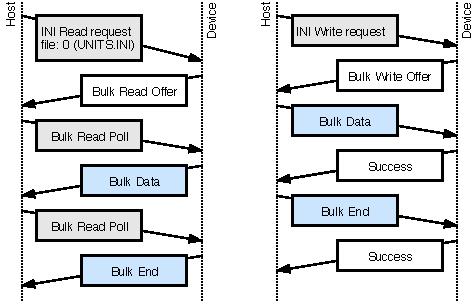
\includegraphics[scale=1.5]{img/bulk-read-write.pdf}
	\caption{\label{fig:bulk-rw}A diagram of the bulk read and write transaction.}
\end{figure}

\subsection{Bulk Read}

To read an INI file, we first send a frame 0x21 (INI Read), specifying the target file in the payload:

\begin{boxedpayload}[INI Read frame structure]
	\cfield{u8} which file to write
		\begin{pldlist}
			\item 0 \dots UNITS.INI
			\item 1 \dots SYSTEM.INI
		\end{pldlist}
\end{boxedpayload}

What follows is a standard bulk read transaction with the requested file.
GEX offers the file for reading with a frame 0x03 (Bulk Read Offer):

\begin{boxedpayload}[Bulk Read frame structure]
	\cfield{u32} full size of the file in bytes
	\cfield{u32} largest chunk that can be read at once
\end{boxedpayload}

Now we can proceed to read the file using 0x04 (Bulk Read Poll), which is always responded to with 0x06 (Bulk Data), or 0x07 (Bulk End) if this was the last frame. Data frames have only the useful data as their payload.

The 0x04 (Bulk Read Poll) payload specifies how many bytes we want to read:

\begin{boxedpayload}[Bulk Read Poll frame structure]
	\cfield{u32} how many bytes to read (at most)
\end{boxedpayload}

\subsection{Bulk Write}

To overwrite an INI file, we first send a frame 0x22 (INI Write) with the file size as its payload. The name of the file is irrelevant, as it's detected automatically by inspecting the content.

\begin{boxedpayload}[INI Write frame structure]
	\cfield{u32} size of the written file, in bytes
\end{boxedpayload}

The write request is confirmed by a frame 0x05 (Bulk Write Offer) sent back:

\begin{boxedpayload}[Bulk Write Offer frame structure]
	\cfield{u32} total bytes to write (here copied from the request frame)
	\cfield{u32} how many bytes may be written per message
\end{boxedpayload}

We can now send the file as a series of frames 0x06 (Bulk Data), or 0x07 (Bulk End) in the last frame, with chunks of the data as their payload. Each frame is confirmed by 0x00 (Success).

\begin{boxedpayload}[Bulk Data or Bulk End frame structure]
	\cfield{u8[]} a chunk of the written file
\end{boxedpayload}

\subsection{Persisting the Changed Configuration to Flash}

The written INI file is immediately parsed and the settings are applied. However, those changes are not persistent: they exist only in RAM and will be lost when the module restarts. To save the current state to Flash, issue a frame 0x23 (Persist Config). This has the same effect as pressing the LOCK button (or replacing the LOCK jumper) when the INI files are edited using the virtual mass storage.

It should be noted that after flashing a firmware, the Flash control registers may remain in an unexpected state and the module must first be manually restarted before attempting to persist settings. Otherwise an assertion will fail and the module is restarted by a watchdog, losing the temporary changes.

% TODO there must be a workaround, and then this paragraph can be removed.


\section{Reading a List of Units}

The frame 0x20 (List Units) requests a list of all available units in the GEX module. The list includes all units' callsigns, names and types. The response payload has the following format (in pseudocode):

\begin{boxedpayload}[List Units response structure (frame type Success)]
	\cfield{u8} the number of available units
	\item For each unit:
		\begin{pldlist}
			\cfield{u8} unit callsign
			\cfield{char[]} unit name (zero-terminated string)
			\cfield{char[]} unit type (zero-terminated string)
		\end{pldlist}
\end{boxedpayload}


\section{Unit Requests and Reports} \label{sec:unit_requests_reports}

Frame types 0x10 (Unit Request) and 0x11 (Unit Report) are dedicated to messages sent to and by unit instances. Each has a fixed header (\textit{inside the payload}) followed by unit-specific data.

\subsection{Unit Requests}

Unit requests deliver a message from the host to a unit instance. Unit drivers implements different commands, each with its own payload structure. The frame 0x10 (Unit Request) has the following structure:

\begin{boxedpayload}[Unit Request frame structure]
	\cfield{u8} unit callsign
	\cfield{u8} command number, handled by the unit driver
	\cfield{u8[]} command payload, handled by the unit driver; its size and content depend on the unit driver and the particular command number
\end{boxedpayload}

The most significant bit of the command byte (0x80) has a special meaning: when set, the message delivering routine responds with 0x00 (Success) after the command completes, unless an error occurred. That is used to get a confirmation that the message was delivered and the module operates correctly (as opposed to e.g. a lock-up resulting in a watchdog reset). Requests which normally generate a response (e.g. reading a value from the unit) should not be sent with this bit set. As a result of this special treatment of the highest bit, there can be only 127 different commands per unit.

\subsection{Unit Reports}

Several unit types can produce asynchronous events, such as reporting a pin change or a triggering condition. The event is timestamped and sent with a frame type 0x11 (Unit Report):

\begin{boxedpayload}[Unit Report (event) frame structure]
	\cfield{u8} unit callsign
	\cfield{u8} report type, defined by the unit driver
	\cfield{u64} event time (microseconds since power-on)
	\cfield{u8[]} report payload; its size and content depend on the unit driver and the particular report type
\end{boxedpayload}

















